\documentclass[serif,aspectratio=169]{beamer}
\usepackage{fontspec,xunicode,xltxtra}
\usepackage{hyperref}
\usepackage{amsmath,amssymb,amsfonts}
\usepackage{graphicx}
\usepackage{wasysym}            % male and female symbols
\usepackage{animate}

\usefonttheme{professionalfonts}

\XeTeXlinebreaklocale zh
\XeTeXlinebreakskip = 0pt plus 1pt minus 0.1pt

\setmainfont{FangSong}
\renewcommand{\baselinestretch}{1.25}

\AtBeginSection[]
{
  \begin{frame}
    \frametitle{目录}  %\insertsection to display section title                                                                             
    \tableofcontents[currentsection]
  \end{frame}
}

\AtBeginSubsection[]
{
  \begin{frame}
    \frametitle{目录}  %\insertsection to display section title                                                                             
    \tableofcontents[currentsubsection]
  \end{frame}
}

\addtobeamertemplate{navigation symbols}{}{%
  \usebeamerfont{footline}%
  \usebeamercolor[fg]{footline}%
  \hspace{1em}%
  \insertframenumber/\inserttotalframenumber
}
%\setbeamercovered{invisible}

\begin{document}

\title{\fontspec{LiSu}第二天 通过系谱和表型记录估计育种值}
\author{于希江}
\date{\tiny{~{二〇一九·十月} \\青岛}}
\institute{挪威生命科学大学畜牧与水产系}
\titlegraphic{
\includegraphics[height=.1\textwidth]{img/nmbu.png}}


\begin{frame}
  \frametitle{第一天回顾}
  \begin{itemize}
  \item 路线图和日程安排
  \item Julia 虚拟环境和 Jupyter notebook 简介
  \item 育种流程简介
  \item 统计模型和育种值
  \item 最小二乘原理
  \item 线性模型最小二乘估计
    \begin{itemize}
    \item 优化估计(模型、目标、优化)
    \item 基因组选择的最小二乘估计
    \item 练习
    \end{itemize}
  \end{itemize}
\end{frame}
    

\frame{
  \titlepage
}

\section{数量性状基因向后代的传递}

\begin{frame}
  \frametitle{数量性状座位 QTL}
  \begin{itemize}
  \item 大多数性状的 QTL 个数 ($N_q$) 通常以千计
  \item 育种中,人们通常只对加性效应感兴趣
    \begin{itemize}
    \item 因为显性和上位效应会在形成配子的过程中分开,在后代中重新组合
    \item 而加性效应是每个等位基因的效应
    \end{itemize}
  \item 个体 $i$ 的育种值 $\displaystyle{\color{red}a_i=\sum_{i=1}^{N_q} x_jb_j}$
  \item 一个后代 $o$ 从个体 $i$ 的 $2N_q$ 个等位基因中抽取 $N_q$ 个
    \begin{itemize}
    \item 于是后代育种值中来自 $i$ 的部分的期望是 $\displaystyle{\color{red}\frac{a_i}{2}}$
    \end{itemize}
  \end{itemize}
\end{frame}


\begin{frame}
  \frametitle{孟德尔抽样误差}
  \begin{itemize}
  \item 由于 QTL 众多,且大小不一,后代 $o$ 很难从个体 $i$ 正好是 $\displaystyle{\color{red}\frac{a_i}{2}}$
  \item 这个由于从众多 QTL 的等位基因抽样所造成的误差 $m$ 叫做{\color{cyan}孟德尔抽样误差}
  \item 这样若 $y_i = \mu + a_i + e_i$,则个体 $i,\, j$ 的后代 $o$ 的表型模型可以写作:
    \begin{itemize}
    \item $y_o = \mu + \frac{a_i}{2} + m_i + \frac{a_j}{2} + m_j + e_o$
    \end{itemize}
  \item $m\sim(0,\,\sigma_m^2)$
    \begin{itemize}
    \item $\sigma_{m_i}^2\approx\sigma_{m_j}^2\approx\frac{\sigma_a^2}{4}$
    \end{itemize}
  \end{itemize}
\end{frame}


\section{多元正态分布和一些情况下遗传力的估计}
\subsection{方差、协方差}
\begin{frame}
  \frametitle{方差、协方差}
  \begin{columns}
    \begin{column}{.5\textwidth}
      \begin{block}{方差($\sigma^2$,或者 Var, V)}
        \begin{itemize}
        \item 方差是对一个随机变量离散 (spread) 程度的度量。
        \item $\sigma^2=\mathrm{E}(X-\mu)^2$
        %\item 离散变量: $\displaystyle\sigma^2=\sum_x(x-\mu)^2\cdot f(x)$
        %\item 连续变量: $\displaystyle\sigma^2=\int_{-\infty}^{\infty}(x-\mu)^2\cdot f(x)dx$
        \item 若由样本估计:$\displaystyle\hat{\sigma}^2=\frac{\sum_{i=1}^n(x_i-\bar{x})^2}{n-1}$
        \end{itemize}
      \end{block}
    \end{column}
    \begin{column}{.5\textwidth}
      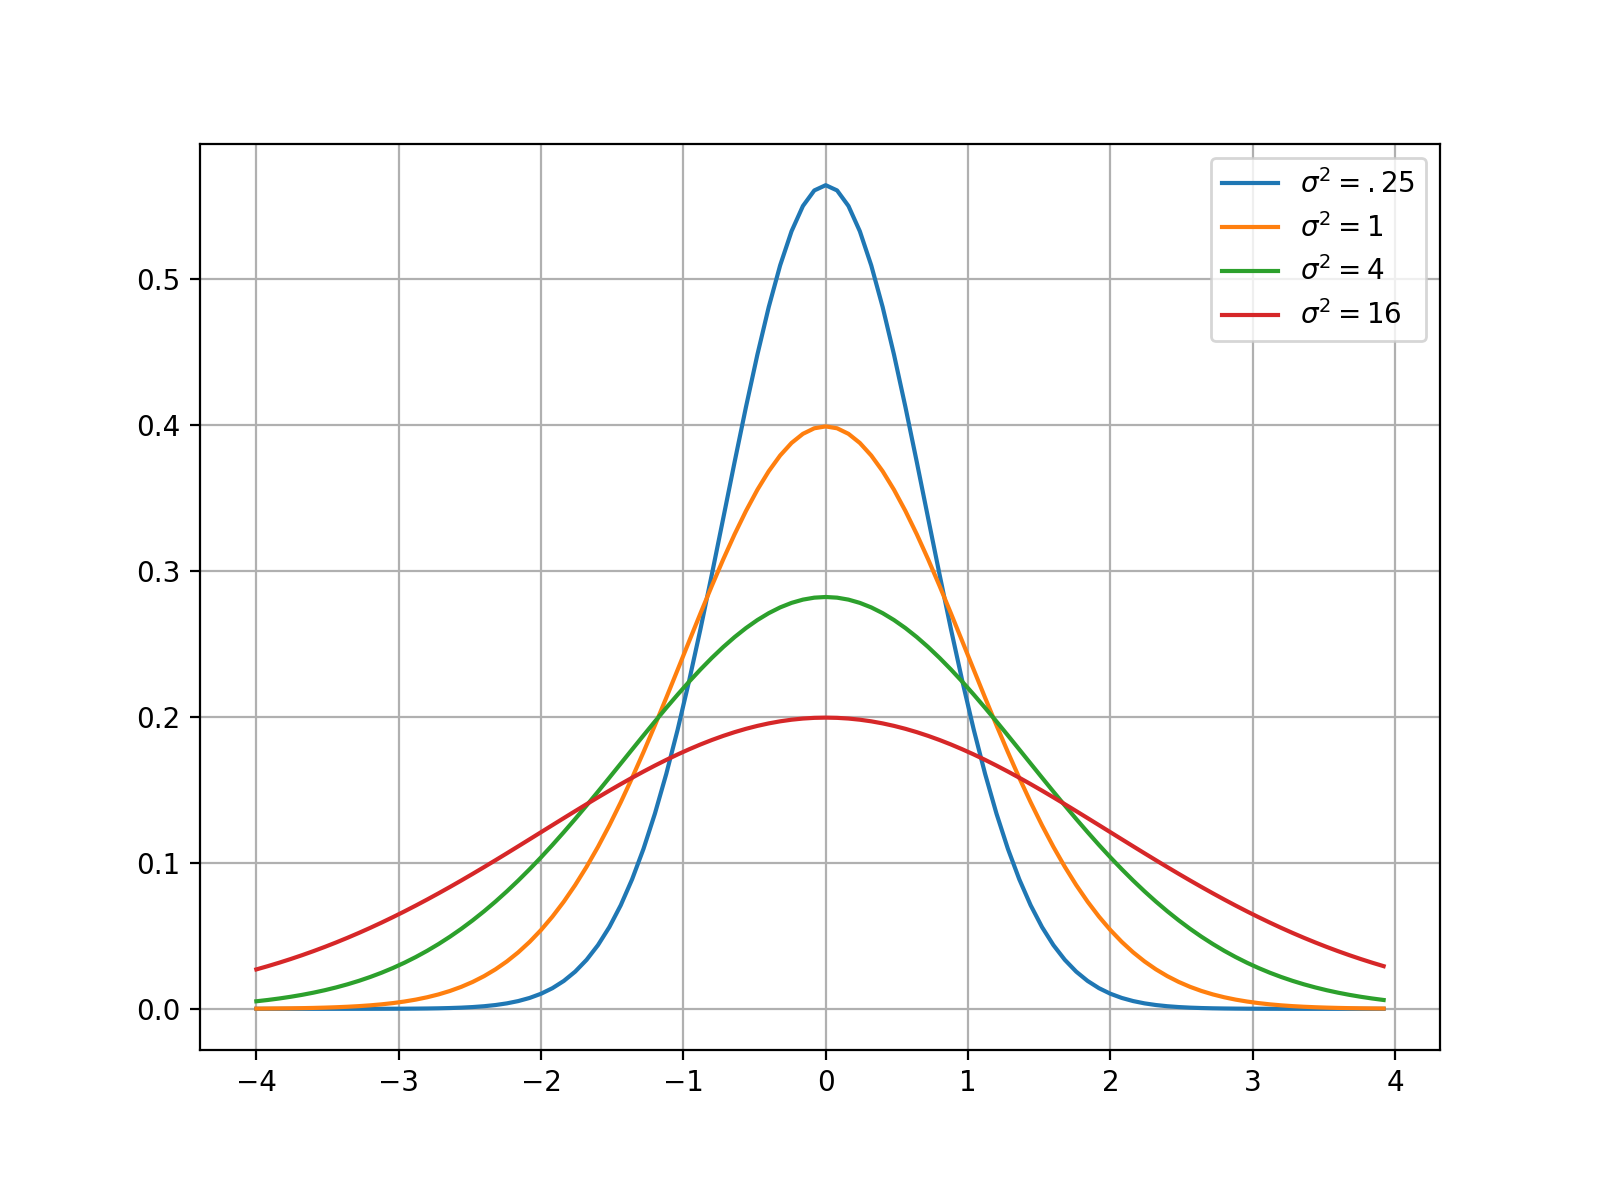
\includegraphics[width=\textwidth]{img/normal-4.png}
    \end{column}
  \end{columns}
\end{frame}


\begin{frame}
  \frametitle{方差、协方差}
  \begin{columns}
    \begin{column}{.5\textwidth}
      \begin{block}{协方差}
        \begin{itemize}
        \item 对两个随机变量协同变化程度的度量
        \item $\mathrm{E}(x_1-\mu_1)(x_2-\mu_2)$
        \item 若由样本估计: $\displaystyle\hat{\sigma}_{12}=\frac{\sum_{i=1}^n(x_{1i}-\mu_1)(x_{2i}-\mu_2)}{n-1}$
        \end{itemize}
      \end{block}
    \end{column}

    \pause
    \begin{column}{.5\textwidth}
      \begin{block}{方差协方差矩阵}
        由 $p$ 个随机数的组成的向量 $\mathbf{x}=[x_1, x_2, ..., x_p]'$,有:
        
        $$
        \Sigma = \left[\begin{array}{llll}
            \sigma_1^2 & \sigma_{12} & \cdots & \sigma_{1p}\\
            \sigma_{21} & \sigma_2^2 & \cdots & \sigma_{2p}\\
            \vdots & \vdots & \ddots & \vdots\\
            \sigma_{p1} & \sigma_{p2} & \cdots & \sigma_p^2
          \end{array}\right]
        $$
        
      \end{block}
    \end{column}
  \end{columns}
\end{frame}


\subsection{多元正态分布}
\begin{frame}
  \frametitle{多元正态分布}
  \begin{columns}
    \begin{column}{.5\textwidth}
      \begin{block}{一元正态分布}
        $$n(x;\mu,\sigma)=\frac{1}{\sigma\sqrt{2\pi}}e^{-\frac{1}{2}\left(\frac{x-\mu}{\sigma}\right)^2}$$
        \begin{description}
        \item [$\mu$] 期望
        \item [$\sigma$] 方差
        \end{description}
      \end{block}
    \end{column}
    
    \pause
    \begin{column}{.5\textwidth}
      \begin{block}{多元正态分布}
        \begin{itemize}
        \item 是一元正态分布的推广
        \end{itemize}

        $$\mathrm{MVN}(\mathbf{x};\mu,\Sigma)=\frac{1}{\sqrt{(2\pi)^p|\Sigma|}}e^{-\frac{1}{2}(\mathbf{x}-\mu)'\Sigma^{-1}(\mathbf{x}-\mu)}$$

        \begin{itemize}
        \item 也记作:$\mathbf{x}\sim\mathrm{MVN}(\mu,\Sigma)$
        \end{itemize}

        $$
        \begin{array}{rcl}
          \mathrm{E}(\mathbf{x}) & = & \mu\\
          \mathrm{Cov}(\mathbf{x}) & = & \Sigma
        \end{array}
        $$
        
      \end{block}
    \end{column}
  \end{columns}
\end{frame}


\begin{frame}
  \frametitle{从两个随机变量来理解方差协方差矩阵}
  \begin{columns}
    \begin{column}{.44\textwidth}
      %convert -coalesce Bivariate41.gif mvn2.png
      %Does not work with evince
      \animategraphics[loop,controls,width=\linewidth]{5}{img/mvn2-}{0}{30}

      \pause
      \begin{itemize}
      \item 右边四图中,每个变量的方差都是 1。
      \end{itemize}
    \end{column}
    
    \begin{column}{.56\textwidth}
      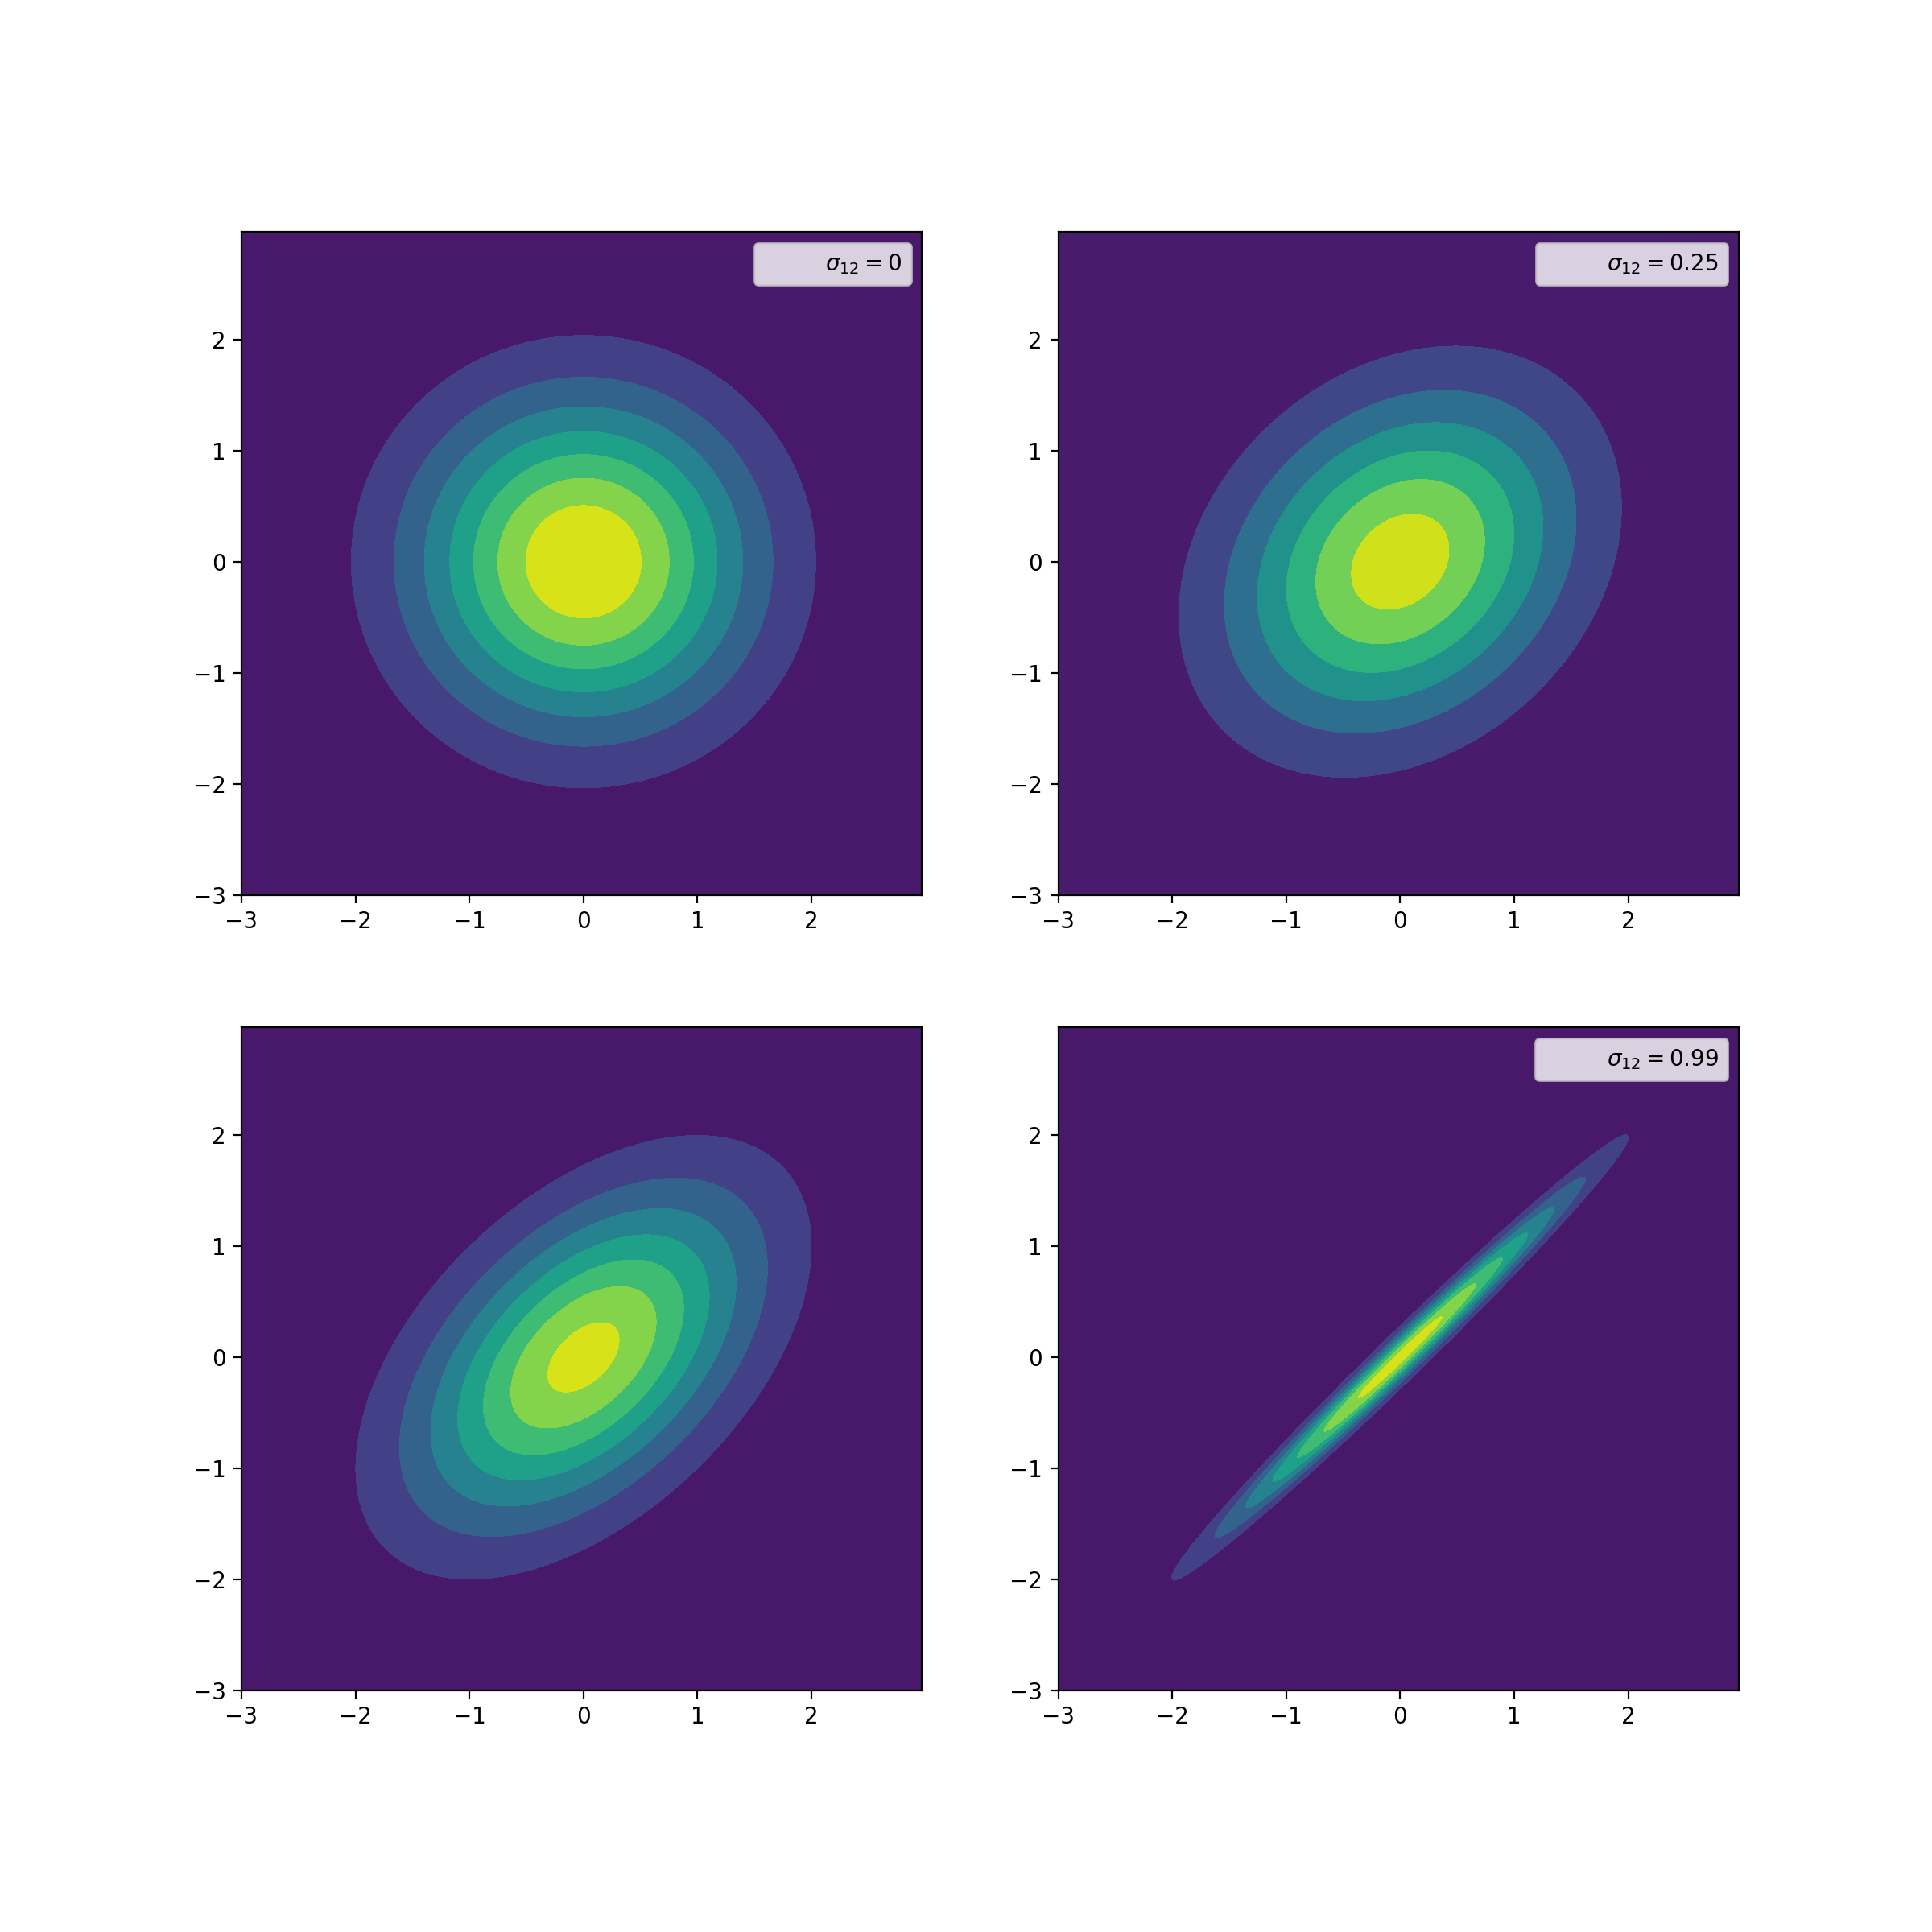
\includegraphics[width=\textwidth]{img/contourf-4.png}
    \end{column}
  \end{columns}
\end{frame}


\subsection{一些情况下遗传力的估计}
\begin{frame}
  \frametitle{半同胞对}
  \begin{columns}
    \begin{column}{.5\textwidth}
      \begin{itemize}
      \item 设半同胞对 $[x_1, x_2]$ 同父异母,则:
        \begin{itemize}
        \item $x_1 = \mu + \frac{a_S}{2} + e$
        \item $x_2 = \mu + \frac{a_S}{2} + e$
          \begin{itemize}
          \item 其中 $e$ 包括其它遗传效应和环境效应。
          \end{itemize}
        \end{itemize}
      \item $\displaystyle\mathrm{Cov}(x_1, x_2) = \frac{\sigma_{a_{S}}^2}{4} = \frac{\sigma_a^2}{4}$
      \item 依模型:$x = \mu+a+e$,每个半同胞变量的方差
        \begin{itemize}
        \item $\mathrm{Var}(x_1)=\mathrm{Var}(x_2)=\sigma_p=\sigma_a^2+\sigma_e^2$
        \end{itemize}
      \end{itemize}

      \end{column}

      \pause
      \begin{column}{.5\textwidth}
        \begin{itemize}
        \item 于是:
        \end{itemize}
        $$
        \left[\begin{array}{c}
            x_1\\
            x_2
          \end{array}
          \right]\sim\mathrm{MVN}
        \left(\left[\begin{array}{c}
            \mu\\
            \mu
          \end{array}
          \right],\,
        \left[
          \begin{array}{cc}
            \sigma_p^2 & \frac{\sigma_a^2}{4}\\
            \frac{\sigma_a^2}{4} & \sigma_p^2
          \end{array}
          \right]
        \right)
        $$
        \begin{itemize}
        \item 注意,此处可见遗传力:
        \end{itemize}
        $$h^2 = \frac{\sigma_a^2}{\sigma_p^2}=\frac{4\cdot\sigma_{12}}{(\sigma_1^2+\sigma_2^2)/2}$$
      \end{column}
  \end{columns}
\end{frame}


\begin{frame}
  \frametitle{半同胞对模拟}
  \begin{columns}
    \begin{column}{.3\textwidth}
      \begin{block}{真值}
        \begin{align*}
          \mu &= \left[\begin{array}{c}0\\0\end{array}\right]\\
          \Sigma & = \left[\begin{array}{cr}1.0 & 0.1\\0.1 & 1.0\end{array}\right]\\
          h^2 & = 0.4
        \end{align*}

        见 {\color{cyan}day-2-mvn.ipynb}.
      \end{block}
    \end{column}

    \pause
    \begin{column}{.7\textwidth}
      \begin{block}{模拟 10 对半同胞}
        \begingroup
        \fontsize{7pt}{7pt}\selectfont
        \begin{tabular}{rrrrrrrrrrr}
          $x_1$&1.2&1.8&0.4&0.2&-1.2&0.1&-2.2&-1.6&-0.0&-0.4\\
          $x_2$&-1.2&0.0&0.2&-1.7&1.1&1.9&-0.3&-2.3&0.7&1.0
        \end{tabular}
        \endgroup
        \begin{align*}
          \hat{\mu} &=\left[\begin{array}{r}-0.2\\-0.1\end{array}\right]\\
          \hat{\Sigma} &=\left[\begin{array}{rr}1.5&0.1\\0.1&1.8\end{array}\right]\\
          \hat{h}^2 &=0.2
        \end{align*}
      \end{block}
    \end{column}
  \end{columns}
\end{frame}


\begin{frame}
  \frametitle{类似的}
  \begin{columns}
    \begin{column}{.5\textwidth}
      \begin{block}{单亲与一子的对}
        \begin{itemize}
        \item 模型
          \begin{itemize}
          \item $y_i=\mu+a_i+e_i$
          \item $y_o=\mu+\frac{a_i}{2}+e_o$
          \end{itemize}
        \item 方差协方差矩阵
          \begin{itemize}
          \item $\Sigma=\left[\begin{array}{cc}\sigma_p^2&\frac{\sigma_a^2}{2}\\\frac{\sigma_a^2}{2}&\sigma_p^2\end{array}\right]$
          \item $h^2=2\cdot\sigma_{12}/\sigma_p^2$
          \end{itemize}
        \end{itemize}
      \end{block}
    \end{column}

    \begin{column}{.5\textwidth}
      \begin{block}{双亲平均与一子}
        \begin{itemize}
        \item 模型
          \begin{itemize}
          \item $y_i=\mu+a_i+e_i$
          \item $y_j=\mu+a_j+e_j$
          \item $(y_i+y_j)/2 = \mu+(a_i+a_j)/2+\bar{e}$
          \item $y_o=\mu+\frac{a_i+a_j}{2}+e_o$
          \end{itemize}
        \item 方差协方差矩阵
          \begin{itemize}
          \item $\Sigma=\left[\begin{array}{cc}\sigma_p^2/2&\sigma_a^2/2\\\sigma_a^2/2&\sigma_p^2\end{array}\right]$
          \item $h^2=\sigma_{12}/\sigma_{\bar{p}}^2$
          \end{itemize}
        \end{itemize}
      \end{block}
    \end{column}
  \end{columns}
\end{frame}


\section{根据系谱和个体表现型估计育种值}
\subsection{引子:一个简单的估计育种值的模型}
\begin{frame}
  \frametitle{简化公牛模型/Sire model}
  \begin{itemize}
  \item 常见于奶牛育种
  \item $p$ 头公牛    
  \item 每头公牛各有 $n_i$ 个女儿
  \item 这样,每个女儿的产奶量模型为
  \end{itemize}
  $$y_{ij} = \mu+u_i+e_{ij}$$
\end{frame}


\subsection{混合模型方程组}
\begin{frame}
  \frametitle{效应/因子}
  \begin{columns}
    \begin{column}{.55\textwidth}
      \begin{block}{几个概念}
        \begin{description}%[labelwidth=\widthof{线性a}]
        \item [线性混合模型] 除随机残差效应,同时包含固定和随机效应的线性模型
        \item [效应] 出现在模型中(右边)的那些量
        \item [固定效应] 效应的所有水平都在样本中出现
        \item [随机效应] 其水平来自更大的抽样空间
        \end{description}
      \end{block}
    \end{column}

    \pause
    \begin{column}{.45\textwidth}
      $$\mathbf{y=Xb+Zu+e}$$

      \begin{block}{其中:}
        \begin{description}
        \item [$\mathbf{y}$] $n\times 1$ 维观测值向量
        \item [$\mathbf{X}$] $n\times s$ 维结构矩阵,或者指示矩阵
        \item [$\mathbf{b}$] $s\times 1$ 个固定效应
        \item [$\mathbf{Z}$] $n\times q$ 维指示矩阵
        \item [$\mathbf{u}$] $q\times 1$ 个随机效应
        \item [$\mathbf{e}$] $n\times 1$ 个随机残差效应
        \end{description}
      \end{block}
    \end{column}
  \end{columns}
\end{frame}


\begin{frame}
  \frametitle{线性混合模型观测值举例}
  \begin{itemize}
  \item 有来自 2 个奶牛场的 2 头公牛的 5 头女儿的记录如下:
  \end{itemize}
  \centering
  \begin{tabular}{rrrr}
    个体号 & 场 & 公牛 & 表型值\\\hline
    1 & 1 & 1 & 11\\
    2 & 1 & 1 & 15\\
    3 & 2 & 1 & 10\\
    4 & 1 & 2 & 19\\
    5 & 2 & 2 & 25
  \end{tabular}
\end{frame}


\begin{frame}
  \frametitle{线性混合模型观测值举例}
  \begin{itemize}
  \item 公牛模型
  \end{itemize}
  $$
  \begin{array}{ccccccccc}
    \mathbf{y} & = & \mathbf{y} & = & \mathbf{Xb} & + & \mathbf{Zu} & + & \mathbf{e}\\
    \left[\begin{array}{c}
        y_{111}\\
        y_{112}\\
        y_{213}\\
        y_{121}\\
        y_{222}
      \end{array}\right] & = &
    \left[\begin{array}{c}
        11\\
        15\\
        10\\
        19\\
        25
      \end{array}\right] & = &
    \left[\begin{array}{cc}
        1 & 0\\
        1 & 0\\
        0 & 1\\
        1 & 0\\
        0 & 1
      \end{array}\right]
    \left[\begin{array}{c}b_1\\b_2\end{array}\right] & + &
    \left[\begin{array}{cc}
        1 & 0\\
        1 & 0\\
        1 & 0\\
        0 & 1\\
        0 & 1
      \end{array}\right]
    \left[\begin{array}{c}u_1\\u_2\end{array}\right] & + &
    \left[\begin{array}{c}
        e_{111}\\
        e_{112}\\
        e_{213}\\
        e_{121}\\
        e_{222}
      \end{array}\right]
  \end{array}
  $$
\end{frame}


\subsection{GLS, BLUE, BLUP}
\begin{frame}
  \frametitle{广义最小二乘 GLS}
  \begin{columns}
    \begin{column}{.5\textwidth}
      \begin{block}{普通最小二乘}
        \begin{itemize}
        \item $e\stackrel{\mathrm{iid}}{\sim}N(0,\sigma_e^2)$
        \item 或者 $\epsilon\sim\mathrm{MVN}(\mathbf{0}, \mathbf{I}\sigma_e^2)$
        \item $\Rightarrow\hat{\mathbf{b}}=(\mathbf{X'X})^{-1}\mathbf{Xy}$
        \end{itemize}
      \end{block}
      \begin{block}{广义最小二乘}
        \begin{itemize}
        \item $\epsilon\sim\mathrm{MVN}(\mathbf{0}, \Sigma)$
        \item 用 $\Sigma^{-1}$ 为观测值加权
          \begin{itemize}
          \item 方差越大,权重越低
          \end{itemize}
        \end{itemize}
      \end{block}
    \end{column}

    \pause
    
    \begin{column}{.5\textwidth}
      \begin{block}{普通最小二乘的优化函数}

        \vspace{-2ex}
        
        $$\mathbf{(y-X\beta)'(y-X\beta)}$$
      \end{block}

      \begin{block}{广义最小二乘的优化函数}

        \vspace{-2ex}
        
        $$(\mathbf{y}-\mathbf{X}\beta)'\Sigma^{-1}(\mathbf{y}-\mathbf{X}\beta)$$
      \end{block}

      \pause
      \begin{block}{$\beta$ 的广义最小二乘估计}

        \vspace{-2ex}
        
        $$\color{red}{\hat{\beta} = (\mathbf{X}'\Sigma^{-1}\mathbf{X})^{-1}\mathbf{X}'\Sigma^{-1}\mathbf{y}}$$
      \end{block}
    \end{column}
  \end{columns}
\end{frame}


\begin{frame}
  \frametitle{OLS 和 GLS 背靠背}
  \begin{columns}
    \begin{column}{.62\textwidth}
      \centering
      \begin{tabular}{rcc}\onslide<1->
        & 普通最小二乘 & 广义最小二乘\\\hline
        模型 & $\mathbf{y=X\beta +\epsilon}$ & $\mathbf{y = X\beta +\epsilon}$\\\\
        分布 & $\epsilon\sim\mathrm{MVN}(\mathbf{0}, \mathbf{I}\sigma_e^2)$ & $\epsilon\sim\mathrm{MVN}(\mathbf{0}, \Sigma)$\\\\
        优化解 & $\hat{\beta}^{\mathrm{OLS}} = $ &  $\hat{\beta}^{\mathrm{GLS}}=$\\
        & $\displaystyle\arg\min_{\beta}\|\mathbf{y-X\beta}\|^2$ & \onslide<3->$\displaystyle\arg\min_{\beta}\|\Sigma^{-1/2}(\mathbf{y-X\beta})\|^2$\\\\ \onslide<4->
        结果 & $\mathbf{(X'X)^{-1}X'y}$ & ${\color{red}(\mathbf{X}'\Sigma^{-1}\mathbf{X})^{-1}\mathbf{X}'\Sigma^{-1}\mathbf{y}}$
      \end{tabular}
    \end{column}
      
    \begin{column}{.38\textwidth}
      \begin{itemize}\onslide<2->
      \item 设有 $\Sigma$ 的平方根 $\Sigma^{1/2}$
      \item $\Sigma = \Sigma^{1/2}\cdot(\Sigma^{1/2})^{\mathrm{T}}$
      \item $\Sigma^{-1} = (\Sigma^{-1/2})^{\mathrm{T}}\cdot\Sigma^{-1/2}$
      \item 则转化模型\\
        $\Sigma^{-1/2}\mathbf{y}=\Sigma^{-1/2}\mathbf{X}\beta+\Sigma^{-1/2}\epsilon$\\
        中
      \item $\mathrm{Var}(\Sigma^{-1/2}\epsilon) = \mathbf{I}\sigma^2$
      \item \onslide<5->$\Sigma^{1/2}$ 通常是 $\Sigma$ 的克莱斯基 (Cholesky) 分解。
      \end{itemize}
      
    \end{column}
  \end{columns}
\end{frame}


\begin{frame}
  \frametitle{关于 GLS 和 OLS}
  \begin{itemize}
  \item GLS 模型其实也可以用 OLS 估计
  \item 但 GLS 估计更好,它考虑了非同质的方差,以及数据内部的相关
  \item 这个结果是好的,因为
    \begin{itemize}
    \item 估计结果是向模型空间的正交投影
    \item 如果 $\Sigma=\mathbf{I}\sigma^2$,则估计结果是最大似然估计。不太严格地说,以最大似然估计结果做参数,观测值的概率最大
    \item 根据高斯-马尔科夫 (Gauss-Markov) 定理,BLUE$(\mathbf{X}\beta) =\mathbf{X}\hat{\beta}$
      %https://en.wikipedia.org/wiki/Gauss%E2%80%93Markov_theorem
    \end{itemize}
  \end{itemize}
\end{frame}


\begin{frame}
  \frametitle{BLUE, BLUP}
  \begin{itemize}
  \item 一般称固定效应的 GLS 估计为 BLUE
  \item 一般称随机效应的 GLS 估计为 BLUP
  \item 混合线性模型:$\mathbf{y=Xb+Zu+e}$
    \begin{itemize}
    \item 平衡设计没有问题
    \item 需要每个家系在各个群体中有分布
    \item 固定效应须要由遗传差异(随机效应)校正
    \item 随机效应须要根据固定效应校正
    \end{itemize}
  \end{itemize}
\end{frame}


\begin{frame}
  \frametitle{混合模型中的方差}
  \begin{align*}
    \mathbf{Y} & = \mathbf{Xb+Zu+e}\\
    \mathrm{Var}(\mathbf{b}) &=\mathbf{0}\\
    \mathrm{Var}(\mathbf{u}) &=\mathrm{E}(\mathbf{uu'}) = \mathbf{G}\\
    \mathrm{Var}(\mathbf{e}) &=\mathrm{E}(\mathbf{ee'}) = \mathbf{R}\\
    \mathrm{Var}(\mathbf{y}) &=\mathrm{Var}(\mathbf{Xb+Zu+e})=\mathbf{ZGZ'+R}
  \end{align*}
\end{frame}


\begin{frame}
  \frametitle{BLUP 的最大似然推导(可选)}
  \begin{columns}
    \begin{column}{.5\textwidth}
      设 $\mathbf{y,u}$ 的联合概率密度为:
      \begin{align*}
        f(\mathbf{y,u}) &=g(\mathbf{y|u})h(\mathbf{u})\\
        g(\mathbf{y|u}) &=g(\mathbf{e})\\
        g(\mathbf{e}) &=\frac{1}{\sqrt{(2\pi)^n|\mathrm{Var}(\mathbf{e})|}}e^{-\frac{1}{2}\mathbf{e}'\mathrm{Var}(\mathbf{e})^{-1}\mathbf{e}}\\
        h(\mathbf{u}) &=\frac{1}{\sqrt{(2\pi)^n|\mathrm{Var}(\mathbf{u})|}}e^{-\frac{1}{2}\mathbf{u}'\mathrm{Var}(\mathbf{u})^{-1}\mathbf{u}}
      \end{align*}
    \end{column}

    \begin{column}{.5\textwidth}
      \begin{align*}
        f(\mathbf{y,u}) & = c_1e^{-\frac{1}{2}\mathbf{e}'\mathbf{R}^{-1}\mathbf{e}}c_2e^{-\frac{1}{2}\mathbf{u}'\mathbf{G}^{-1}\mathbf{u}}\\
        & = ce^{-\frac{1}{2}\mathbf{e}'\mathbf{R}^{-1}\mathbf{e}}e^{-\frac{1}{2}\mathbf{u}'\mathbf{G}^{-1}\mathbf{u}}\\
        L &= f(\mathbf{y,u})\\
        \log(L) &=\log(c)-\frac{1}{2}\mathbf{e}'\mathbf{R}^{-1}\mathbf{e}-\frac{1}{2}\mathbf{u}'\mathbf{G}^{-1}\mathbf{u}
      \end{align*}
    \end{column}
  \end{columns}
\end{frame}


\begin{frame}
  \frametitle{BLUP 的最大似然推导(续)}
  \begin{align*}
    \log(L) &=\log(c)-\frac{1}{2}\mathbf{e}'\mathbf{R}^{-1}\mathbf{e}-\frac{1}{2}\mathbf{u}'\mathbf{G}^{-1}\mathbf{u}\\
    \mathbf{e} &=\mathbf{y-Xb-Zu}\\
    \log(L) &=\log(c)\\
    &\quad-\frac{1}{2}(\mathbf{y-Xb-Zu})'\mathbf{R}^{-1}(\mathbf{y-Xb-Zu})\\
    &\quad-\frac{1}{2}\mathbf{u}'\mathbf{G}^{-1}\mathbf{u}\\
  \end{align*}
\end{frame}

\begin{frame}
  \frametitle{BLUP 的最大似然推导 -- 结果}
  令 $\displaystyle\frac{\partial(\log L)}{\partial\mathbf{b}}=\frac{\partial(\log L)}{\partial\mathbf{u}}=0$,得混合模型方程组

  \vspace{2em}
  
  $$
  \color{red}\left[\begin{array}{ll}
      \mathbf{X}'\mathbf{R}^{-1}\mathbf{X} & \mathbf{X}'\mathbf{R}^{-1}\mathbf{Z}\\
      \mathbf{Z}'\mathbf{R}^{-1}\mathbf{X} & \mathbf{Z}'\mathbf{R}^{-1}\mathbf{Z}+\mathbf{G}^{-1}
    \end{array}\right]
  \left[\begin{array}{cc}
      \hat{\mathbf{b}}\\
      \hat{\mathbf{u}}
    \end{array}\right] = 
  \left[\begin{array}{c}
      \mathbf{X}'\mathbf{R}^{-1}\mathbf{y}\\
      \mathbf{Z}'\mathbf{R}^{-1}\mathbf{y}
    \end{array}\right]
  $$
  
\end{frame}


\begin{frame}
  \frametitle{BLUP 的特殊情形}
  \begin{columns}
    \begin{column}{.5\textwidth}
      \begin{block}{$\mathbf{R=I}\sigma_e^2$}

        $$
        \color{cyan}\left[\begin{array}{ll}
            \mathbf{X}'\mathbf{X} & \mathbf{X}'\mathbf{Z}\\
            \mathbf{Z}'\mathbf{X} & \mathbf{Z}'\mathbf{Z}+\mathbf{G}^{-1}\sigma_e^2
          \end{array}\right]
        \left[\begin{array}{cc}
            \hat{\mathbf{b}}\\
            \hat{\mathbf{u}}
          \end{array}\right] = 
        \left[\begin{array}{c}
            \mathbf{X}'\mathbf{y}\\
            \mathbf{Z}'\mathbf{y}
          \end{array}\right]
        $$
        
      \end{block}
    \end{column}

    \begin{column}{.5\textwidth}
      \begin{block}{由 $\mathbf{G}^{-1}=\mathbf{A}^{-1}\sigma_u^{-2}$ 和 $\lambda=\frac{\sigma_e^2}{\sigma_u^2}$}

        $$
        \color{cyan}\left[\begin{array}{ll}
            \mathbf{X}'\mathbf{X} & \mathbf{X}'\mathbf{Z}\\
            \mathbf{Z}'\mathbf{X} & \mathbf{Z}'\mathbf{Z}+\mathbf{A}^{-1}\lambda
          \end{array}\right]
        \left[\begin{array}{cc}
            \hat{\mathbf{b}}\\
            \hat{\mathbf{u}}
          \end{array}\right] = 
        \left[\begin{array}{c}
            \mathbf{X}'\mathbf{y}\\
            \mathbf{Z}'\mathbf{y}
          \end{array}\right]
        $$
        
      \end{block}
    \end{column}
  \end{columns}
  \tiny{注:逆矩阵的计算量 $(O(n^3))$ 比矩阵相乘 $(O(n^2))$ 高很多,而通常 G 的维度远少于观测值的个数。因而其逆矩阵计算比观测值方差的逆矩阵容易得多。}
\end{frame}


\begin{frame}
  \begin{columns}
    \begin{column}{.5\textwidth}
      \begin{block}{小结}
        \begin{itemize}
        \item 微效等位基因向后代的传递
        \item 方差、协方差
        \item 多元正态分布
        \item 广义最小二乘的原理
        \item BLUE 是固定效应的广义最小二乘估计
        \item BLUP 和混合线性方程组
        \end{itemize}
      \end{block}
    \end{column}

    \pause
    \begin{column}{.5\textwidth}
      \begin{block}{下一节}
        \begin{itemize}
        \item A 矩阵
        \item A 的逆矩阵
        \item 几种在育种中常用的模型
        \item 模拟和计算
        \end{itemize}
      \end{block}
    \end{column}
  \end{columns}
\end{frame}
\end{document}
